\documentclass[14pt, a4paper]{article}
\usepackage{float}
\usepackage{graphicx}
\usepackage[utf8]{inputenc}

\DeclareGraphicsExtensions{.png}

\begin{document}

%\title and intnro
\begin{titlepage}
	\begin{center}
		
		\begin{figure}[t]
			\centerline{
			
\includegraphics[width=450px]{./Graphics/KPTH_Logo.png}}
		\end{figure}		
		
		\textbf{\LARGE Gynaecological Patient Information
		management System:}
		
		\vspace{1 cm}
	    \textbf{\LARGE \\User Manual}
		
		\vspace{1 cm}
		\LARGE{\textbf{Team Pentec: }}
		

		\begin{flushright} \large
			
			Ruth Ojo 12042804\newline
			Liz Joseph 10075268\newline
			Trevor Austin 11310856\newline
			Maria Qumayo 29461775\newline
			Lindelo Mapumulo 12002862\newline
		\end{flushright}
		
				\vspace{1 cm}
				\centering
				
\includegraphics[width=150px]{./Graphics/Pentec_Logo.png}

		
		{\LARGE Version 1.4} 
		\\
		{\large \today}		
		
		
	\end{center}
\end{titlepage}


\begin{abstract}
\Large
This document is the Software User Manual (SUM) for the Patient Information Management System project and was made according to the software engineering standard described in the tender proposal provided by Professor Snyman. The Software User Manual (SUM) instructs how to install and use the
Patient Information Management System software. This project is part of the Software Engineering Project course (COS301) at the University of Pretoria.\\
\end{abstract}

\newpage

%\table of content
\tableofcontents
\newpage

\section{Introduction}


\subsection{Change Log}
Document Title: Software User Manual\\
Version: 0.1.0\\
Document Status: conditionally approved\\
Version Date Author(s) Summary\\
0.0.1 29-05-2015 LN. Joseph Document creation\\


\subsection{Intended readership}
This document covers the use for the following users of the PIMS system:\\
\begin{description}
\item the system administrator
\item the project administrators
\item the medical staff
\item the usability test subjects
\end{description}

\subsection{Applicability}
This Software User Manual (SUM) applies to the PIMS software, version 0.1.\\


\subsection{Purpose}
The purpose of the SUM is to assist the user in installing and using the PIMS software.\\

	
\subsection{How to use this document}
\begin{description}
\item How it is to be used:
\item[$\bullet$] Title page - System name and the names and/or affiliation of all stakeholders.
\item[$\bullet$] Introduction - Introduction to the System
\item[$\bullet$] Overview - Purpose of the system
\item[$\bullet$] Configuration - Configuration used by the system
\item[$\bullet$] Installation - Detailed description of where to find the software and how to install it.
\item[$\bullet$] Getting Starting - Walk through of the system
\item[$\bullet$] Using the System - Description of the systems functions
\item[$\bullet$] Troubleshooting - Procedures to take in case of errors
\end{description}

	
\subsubsection{Problem Reporting}
Since the Pentec team will be dissolved after completion of the PIMS project, the
issue of problem reporting is left to the Administrator, Professor Snyman.\\
	
	
\newpage

\section{Overview}
The purpose of this software is to be used by doctors and medical staff. It allows the administrative users to electronically fill in medical forms and be able to query for statistics for those forms and eventually receive a prediction that could assist in the functionality of the Kalafong Hospital. Regular users are allowed to fill in medical forms.
\\

\newpage

\section{Configuration}
\section{System Configuration}
\subsection{Basic System Structure}
The current system that is in place makes use of a Node.js server that interacts with any web client. The server is hosted through a PaaS named Heroku. The system delivers compiled jade files to the users that are stylized using CSS. The jade files are controlled and animated by Javascript and jQuery. The node.js server accesses MongoDB database hosted on the DaaS, mongolab. This is illustrated below:
\begin{figure}[h!]
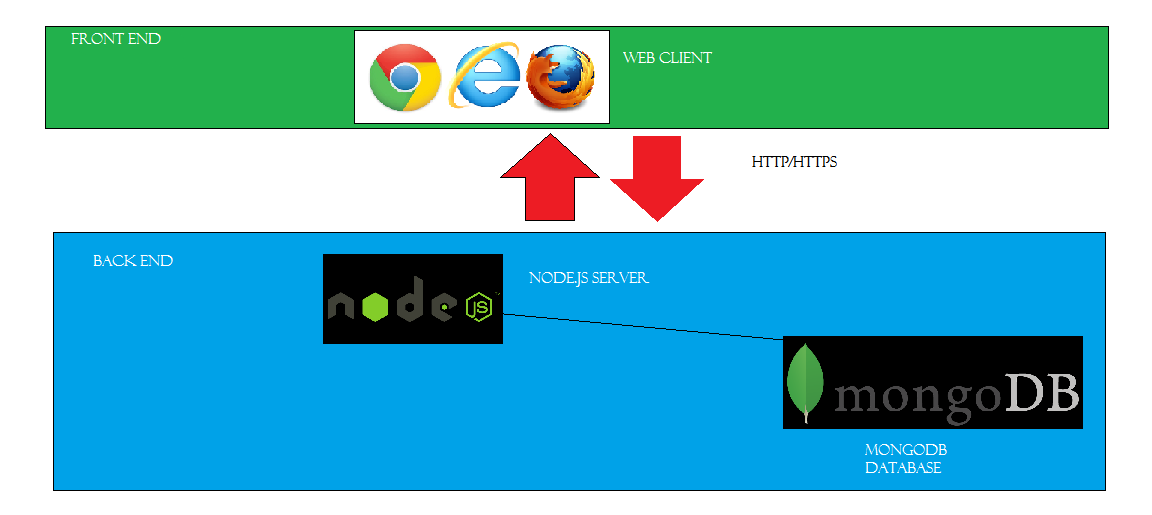
\includegraphics[width=1.0\textwidth]{Graphics/Screenshots/infrastructure}
\end{figure}
\newpage
\subsection{Node.js Architecture}
Node.js is an asynchronous langauge and its basic client-server communication is illlustrated below:
\begin{figure}[h!]
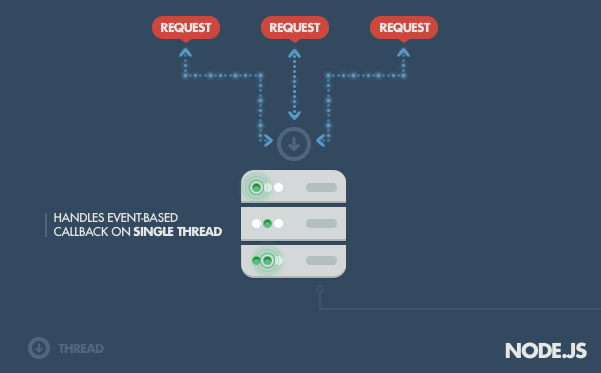
\includegraphics[width=1.0\textwidth]{Graphics/Screenshots/nodejsinfrastructure}
\end{figure}
\subsection{Communication Protocols Used}
This is the current list of all communication protocols used by PIMS:
\begin{itemize}
	\item HTTP/HTTPS
	\item SMTP
\end{itemize}
\newpage

\newpage


\section{Installation}
\subsection{Running the Software}
\begin{enumerate}
  \item Website page
  \begin{enumerate}
  \item Establish an internet connection
    \item Search for website in web browser
    \item Log into PIMS system with given authentication codes
  \end{enumerate}
  \item Mobile Application
   \begin{enumerate}
   \item Establish an internet connection
    \item Search for website in web browser
    \item Log into PIMS system with given authentication codes
  \end{enumerate}
  \item Tablet or other
   \begin{enumerate}
\item Establish an internet connection  
    \item Search for website in web browser
    \item Log into PIMS system with given authentication codes
  \end{enumerate} \ldots
\end{enumerate}

\subsection{Shutting down the website}
Contact your service provider(hosting site) to pull down the software
\newpage


\section{Getting Started}
\subsection{Systems Procedure Order}
This section describes a brief overview of how a user can access the system, it shows perspectives from an adminstrative user as well as normal users. The sections that are discussed can be found in more detail in the next section.
\subsection{Splash Page}
\subsection{Login}
\subsection{Navbar}
\subsection{Home Icons}
\subsection{Fill Forms}
\subsection{Statistics}
\subsection{Add User}
\subsection{Update Profile}
\subsection{Logout}
\newpage



\section{Using the System}
\begin{description}
\item The login, forms, user and statistics operations are described in this chapter.
\end{description}


\subsection{User}
	  
\subsubsection{add user}
\begin{description}
\item [Functional Description] This operation adds a user to the PENTEC-PIMS database.
\item [Formal Description] \hfill
\begin{itemize}
	\item Syntax: add user (username,surname,password,staff type,department,email address,user right) as [Users] [A schema to save the details of all medical staff that can access the system]\\
	\item Parameters:
		\begin{itemize}
			\item [schema] (Required when chosen) : Users Schema\\
			\item [pentec\_pims] (Required) : This is the name of the database in mongoose that we are using\\
			\item [details](Required):All the above mentioned details in syntax are important to add a user\\
		 \end{itemize}
\end{itemize}
\item[Examples]\hfill
\begin{itemize}
	\item add user John Doe, Medical Intern, User right 2, Gynaecologist
	\item add user url:http://kalafongpims.herokuapp.com/addUser
	\item URL : :http://kalafongpims.herokuapp.com as Medical Staff This is a medical research dataset PENTEC Software User Manual 0.1.0 14
\end{itemize}
\item[Possible errors]\hfill
	\begin{itemize}
	\item You do not have the login creditials
	\item A user with name [username]already exists
	\item You don't have the role of admin
	\end{itemize}
\item[Solutions]\hfill
	\begin{itemize}
	\item Go to admin(Dr Snyman) and request he add you to the database of users.
	\item Register with your already given details. No duplicates allowed.
	\item  Go to admin(Dr Snyman) and request he make you admin.
	\end{itemize}
\item[Related operations] remove user
\end{description}
	  
\subsubsection{edit profile}
\begin{description}
\item[Functional Description] This operation edits a users profile and saves it to the PENTEC-PIMS database.
\item[Formal description]\hfill
\begin{itemize}
	\item Syntax: edit user (username,surname,password,confirm password,staff type,department,email address,user right) as [Users] [A schema to save the details of all medical staff that can access the system]\\
	\item Parameters:
		\begin{itemize}
			\item [schema] (Required when chosen) : Users Schema
			\item [pentec\_pims] (Required) : This is the name of the database in mongoose that we are using.
			\item [details] (Required) :All the above mentioned details in syntax are important to complete edit profile.
		\end{itemize}
\end{itemize}

\item[Examples]\hfill
\begin{itemize}
	\item edit user John Doe, Medical Intern, User right 2, Gynaecologist
	\item edit user url:http://kalafongpims.herokuapp.com/editProfile
	\item URL : :http://kalafongpims.herokuapp.com as Medical Staff This is a medical research dataset PENTEC Software User Manual 0.1.0 14
\end{itemize}

\item[Possible errors]\hfill
\begin{itemize}
	\item You do not have the login creditials to log into the system
	\item Passwords don't match
	\item You don't have the role of admin
	\item You do not appear on the system
\end{itemize}

\item[Solutions]\hfill
\begin{itemize}
	\item Go to admin(Dr Snyman) and request he add you to the database of users.
	\item Register with your already given details sent to your email. No duplicates allowed.
	\item Re-enter your password
	\item  Go to admin(Dr Snyman) and request he make you admin.
\end{itemize}
\item[Related operations] add user
\end{description}
		   
\subsubsection{password}
\begin{description}
\item[Functional description] This operation changes your password on the PENTEC-PIMS database.
\item[Formal description]\hfill
\begin{itemize}
	\item Syntax:password (confirm password, password) as [Users] [A schema to save the details of all medical staff that can access the system]\\
	\item Parameters:
	\begin{itemize}
		\item [schema] (Required when chosen) : Users Schema
		\item [pentec\_pims] (Required) : This is the name of the database in mongoose that we are using.
		\item [details] (Required) :All the above mentioned details in syntax are important to complete password.
	\end{itemize}
\end{itemize}

\item[Examples]\hfill
\begin{itemize}
	\item password mysecretpassword, mysecretpassword
	\item add user url:http://kalafongpims.herokuapp.com/editProfile
	\item URL : :http://kalafongpims.herokuapp.com as Medical Staff This is a medical research dataset
	PENTEC Software User Manual 0.1.0 14
\end{itemize}
\item[Possible errors]\hfill
\begin{itemize}
	\item You do not have the login creditials
	\item You don't have the role of admin
	\item Passwords dont match
\end{itemize}
\item[Solutions]\hfill
\begin{itemize}
	\item Go to admin(Dr Snyman) and request he add you to the database of users.
	\item  Go to admin(Dr Snyman) and request he make you admin.
	\item Re-enter your password carefully.
\end{itemize}
\item[Related operations] none
\end{description}

\subsubsection{list for}
\begin{description}
\item[Functional description] This operation list all the available forms in the PENTEC-PIMS database.
\item[Formal description]\hfill
\begin{itemize}
	\item Syntax: list form (form name) as [Forms] [A schema to save the details of all medical forms in the system]\\
	\item Parameters:
	\begin{itemize}
		\item [schema] (Required when chosen) : Forms Schema
		\item [pentec\_pims] (Required) : This is the name of the database in mongoose that we are using.
		\item [details] (Required) :All the above mentioned details in syntax are important to complete list form.
	\end{itemize}
\end{itemize}

\item[Examples]\hfill
\begin{itemize}
	\item list form Gynaecology Form
	\item list form url:http://kalafongpims.herokuapp.com/forms
	\item URL : :http://kalafongpims.herokuapp.com as Medical Staff This is a medical research dataset
	PENTEC Software User Manual 0.1.0 14
\end{itemize}

\item[Possible errors]\hfill
\begin{itemize}
	\item You do not have the login creditials
	\item The form you are looking for does not exist
\end{itemize}

\item[Solutions]\hfill
\begin{itemize}
	\item Go to admin(Dr Snyman) and request he add you to the database of users.
	\item Go to admin(Dr Snyman) and request he create the form.
\end{itemize}
\item[Related operations] none

\end{description}
	      	      
	      
\subsubsection{save form}
\begin{description}
\item[Functional description] This operation allows you to save a form to the PENTEC-PIMS database.
\item [Formal description]\hfill
\begin{itemize}
	\item Syntax: save form (data, form name) as [Forms] [A schema to save the details of all forms created in the system]\\
	\item Parameters:
	\begin{itemize}
		\item [schema] (Required when chosen) : Forms Schema
		\item [pentec\_pims] (Required) : This is the name of the database in mongoose that we are using.
		\item [details] (Required) :All the above mentioned details in syntax are important to complete save form.
	\end{itemize}
\end{itemize}

\item[Examples]\hfill
\begin{itemize}
	\item save form discharge form, JSON Object
	\item save form url:http://kalafongpims.herokuapp.com/formbuilder
	\item URL : :http://kalafongpims.herokuapp.com as Medical Staff This is a medical research dataset
	PENTEC Software User Manual 0.1.0 14
\end{itemize}

\item[Possible errors]none
\item[Solutions] none
\item [Related operations] list form, add form
\end{description}

\subsubsection{send notification}
\begin{description}
\item[Functional description] This operation allows you to notify a patient of their follow up via email.
\item[Formal description]\hfill
\begin{itemize}
	\item Syntax: add notification (username, email, message, date) as [Users] [A schema to save the details of all medical staff that can access the system]\\
	\item Parameters:
	\begin{itemize}
		\item [schema] (Required when chosen) : Users Schema
		\item [pentec\_pims] (Required) : This is the name of the database in mongoose that we are using.
		\item [details] (Required) :All the above mentioned details in syntax are important to complete send notification.
	\end{itemize}
\end{itemize}
\item[Examples]\hfill
\begin{itemize}
	\item add notification John Doe,john@gmail.com, "John Please come for your checkup",2015
	\item add notification url:http://kalafongpims.herokuapp.com/sendNotification
	\item URL : :http://kalafongpims.herokuapp.com as Medical Staff This is a medical research dataset
	PENTEC Software User Manual 0.1.0 14
\end{itemize}

\item[Possible errors]\hfill
\begin{itemize}
	\item You cant find the users name
	\item User does not have an email address
\end{itemize}


\item[Solutions]\hfill
\begin{itemize}
	\item Patient does not exist in the system
	\item Notification cannot be sent to user
\end{itemize}


\item[Related operations] remove user
\end{description}
	   
\subsubsection{list department}
\begin{description}
\item[Functional description] This operation lists all the departments on the splash screen from the PENTEC-PIMS database.
\item[Formal description]\hfill
\begin{itemize}
	\item Syntax: list department (name of department, link) as [Departments] [A schema to save the details of all departments in the system and display them on the splash screen]\\
	\item Parameters:
	\begin{itemize}
		\item [schema] (Required when chosen) : Departments Schema
		\item [pentec\_pims] (Required) : This is the name of the database in mongoose that we are using.
		\item [details] (Required) :All the above mentioned details in syntax are important to complete list user.
	\end{itemize}
\end{itemize}

\item[Examples]\hfill
\begin{itemize}
	\item list department Gynaecology, www/d/
	\item list department url:http://kalafongpims.herokuapp.com/splash
	\item URL : :http://kalafongpims.herokuapp.com as Medical Staff This is a medical research dataset
	PENTEC Software User Manual 0.1.0 14
\end{itemize}
\item[Possible errors] None
\item[Solutions] None
\item[Related operations] none
\end{description}
	      
\subsubsection{exit}
\begin{description}
\item[Functional description] This operation adds a user to the PENTEC-PIMS database.
\item[Formal description]\hfill
\begin{itemize}
	\item Syntax: add user (none) as [none] [none]\\
	\item Parameters:
	\begin{itemize}
		\item [schema] (Required when chosen) : Users Schema
		\item [pentec\_pims] (Required) : This is the name of the database in mongoose that we are using.
		\item [details] (Required) :All the above mentioned details in syntax are important to complete exit.
	\end{itemize}
\end{itemize}

\item[Examples]\hfill
\begin{itemize}
	\item exit [press logout button]
	\item exit url:http://kalafongpims.herokuapp.com/home
	\item URL : :http://kalafongpims.herokuapp.com as Medical Staff This is a medical research dataset
	PENTEC Software User Manual 0.1.0 14
\end{itemize}

\item[Possible errors] none
\item[Solutions] none
\item [Related operations] login
\end{description}

\subsection{Login}
\subsubsection{authenticate} 
\begin{description}
\item[Functional Description] This function authenticates a user and logs them into the system.
\item[Formal Description]\hfill
\begin{itemize}
	\item Syntax: authenticate([username], [password], [callback])\\
	\item Parameters:
		\begin{itemize}
			\item [username] (Required): This is the username of the user, it will usually be the user's name or a unique number assigned to them.
			\item [password] (Required): This is the password of the user and is used to authenticate the user.
			\item [callback](Opitional): This is the callback function and is used to keep the processes synchronous.
		\end{itemize}
\end{itemize}
\item[Examples]\hfill
\begin{itemize}
	\item authenticate("John", 1234)
	\item authenticate("john", 1234, thisIsAFunction(){})
\end{itemize}
\item[Possible Errors \&  Solutions]\hfill
	\begin{itemize}
		\item Problem: Your login does not exist.
		\item Solution: Contact supervisor.
		\item Problem: Your password is incorrect.
		\item Solution: Contact supervisor.
		\item Problem: You are trying to access an admin page but it takes you to a regular user page.
		\item Solution: Request supervisor to change your rank.
	\end{itemize}
\item [Related operations]	checkAdmin
\end{description}

\subsubsection{check admin}
\begin{description}
\item[Functional Description] Determines if the user is an administrator.
\item[Formal Description]\hfill
\begin{itemize}
	\item Syntax: checkAdmin([username], [password], [callback])\\
	\item Parameters:
		\begin{itemize}
			\item [username] (Required): This is the username of the user, it will usually be the user's name or a unique number assigned to them.
			\item [password] (Required): This is the password of the user and is used to authenticate the user.
			\item [callback](Opitional): This is the callback function and is used to keep the processes synchronous.
		\end{itemize}
\end{itemize}
\item[Examples]\hfill
\begin{itemize}
	\item checkAdmin("John", 1234)
	\item checkAdmin("john", 1234, thisIsAFunction(){})
\end{itemize}
\item[Possible Errors \& Solutions]
\begin{itemize}
	\item Problem: You are trying to access an admin page but takes you to a regular user page.
	\item Solution: Request supervisor to change your rank.
\end{itemize}
\item[Related operations] authenticate
\end{description}

\subsubsection{recaptcha}
\begin{description}
\item[Functional Description] This function is a security feature to ensure the user is not an automated bot or machine.
\item[Formal Description]\hfill
\begin{itemize}
	\item Syntax: recapture([action], [callback])\\
	\item Parameters:
		\begin{itemize}
			\item [action] (Required): This is the action taken by the user in the form of a check on the checkbox.
			\item [callback](Opitional): This is the callback function and invoked by the click event and allows the user to log into the system.
		\end{itemize}
\end{itemize}
\item[Examples]\hfill
\begin{itemize}
	\item recaptcha(event(Click), thisIsACallbackFunction(){//allow user to log in})
\end{itemize}
\item[Possible Errors \& Solutions]
\begin{itemize}
	\item Problem: Error message "Please check the recaptcha box before logging in"
	\item Solution: Locate the recaptcha box at the bottom of the log in box and click it.
\end{itemize}
\item[Related operations] authenticate
\end{description}


\subsection{Statistics}

\subsubsection{get daterange}
\begin{description}
\item[Functional Description] This function allows the user to select a time period that he would like his data to reflect.
\item[Formal Description]/hfill
\begin{itemize}
	\item Syntax: getDatarange([startDate], [endDate], [callback])\\
	\item Parameters:
		\begin{itemize}
			\item [startDate](Required) This is the start date that has been selected.
			\item [endDate](Required) This is the end date that has been selected.
			\item [callback](Optional) This is the callback function and is used to keep the processes synchronous.
		\end{itemize}
\end{itemize}
\item[Examples]\hfill
\begin{itemize}
	\item getDatarange({startDate : "10/10/2014", endDate: "10/10/2015"})
	\item getDatarange({startDate : "10/10/2014", endDate: "10/10/2015"}, callback)
\end{itemize}
\item[Possible Errors \& Solutions]
\begin{itemize}
	\item Problem: No date selected
	\item Solution: Reselect the date on the date time picker and click apply then select other procedures and click query.
	\item Problem: No procedures in the dates selected
	\item Solution: Graph will show user there are no procedures in that period.
\end{itemize}
\item[Related operations] \hfill
\begin{itemize}
	\item get interval
	\item get graph
\end{itemize}
\end{description}

\subsubsection{get interval}
\begin{description}
\item[Functional Description] This function gets the interval based data in the dropdownlist and certain selectors and uses it to query the database.
\item[Formal Description]/hfill
\begin{itemize}
	\item Syntax: getInterval([selectors], [callback])\\
	\item Parameters:
		\begin{itemize}
			\item [interval][statistics],[selectors](Required) These are the selectors put in place to customize the procedures that are selected.
			\item [callback](Required) This is the callback function and is used to keep the processes synchronous.
		\end{itemize}
\end{itemize}
\item[Examples]\hfill
\begin{itemize}
	\item getInterval(Weekly,Average Age,{startDate : "10/10/2014", age: 25, endDate: "10/10/2015"})
	\item getInterval(Yearly, Average Age,{startDate : "10/10/2014", age: 25, endDate: "10/10/2015"}, callback)
\end{itemize}
\item[Possible Errors \& Solutions]
\begin{itemize}
	\item Problem: Invalid selectors
	\item Solution: Choose a valid selector.
	\item Problem: No operations during that selector
	\item Solution: Graph will correctly depict the scenario.
\end{itemize}
\item[Related operations] \hfill
\begin{itemize}
	\item get daterange
	\item get graph
\end{itemize}
\end{description}

\subsubsection{get graph}

\begin{description}
\item[Functional Description] This function gets data selected from the input boxes and after querying the database returns them in a format which can be converted into a graph.
\item[Formal Description]/hfill
\begin{itemize}
	\item Syntax: getGraph([startDate],[endDate],[interval],[statistic], [callback])\\
	\item Parameters:
		\begin{itemize}
			\item [startDate](Required) This is the start date that has been selected.
			\item [endDate](Required) This is the end date that has been selected.
			\item [interval](Required) This is the interval that has been selected.
			\item [statistic](Required) This is the statistic that has been selected.
			\item [callback](Optional) This is the callback function and is used to keep the processes synchronous.
		\end{itemize}
\end{itemize}
\item[Examples]\hfill
\begin{itemize}
	\item getGraph({startDate : "10/10/2014", procedure: "all", endDate: "10/10/2015"},"Weekly", "Average Age", )
	\item getGraph({startDate : "10/10/2014", procedure: "all" ,endDate: "10/10/2015"}, callback)
\end{itemize}
\item[Possible Errors \& Solutions]
\begin{itemize}
	\item Problem: Data does not exist
	\item Solution: Graph shows the appropriate message.
	\item Problem: Invalid selectors
	\item Solution: Choose a valid selector.
\end{itemize}
\item[Related operations] \hfill
\begin{itemize}
	\item get interval
	\item get datarange
\end{itemize}
\end{description}

\subsubsection{get statistics}
\begin{description}
\item[Functional Description] This function allows the user to select a specific statistic he would like his data to reflect.
\item[Formal Description]/hfill
\begin{itemize}
	\item Syntax: getStatistics([stats], [callback])\\
	\item Parameters:
		\begin{itemize}
			\item [stats](Required) This is the statistics that has been selected.
			\item [callback](Optional) This is the callback function and is used to keep the processes synchronous.
		\end{itemize}
\end{itemize}
\item[Examples]\hfill
\begin{itemize}
	\item getStatistics({stats:"Elective Procedures"})
\end{itemize}
\item[Possible Errors \& Solutions]
\begin{itemize}
	\item Problem: No statistic value selected
	\item Solution: Error message asking you to select a statistic value will show.
	\item Problem: No procedures in the dates selected
	\item Solution: Graph will show user there are no procedures in that period and ask you to select dates.
\end{itemize}
\item[Related operations] \hfill
\begin{itemize}
	\item get interval
	\item get graph
	\item get daterange
\end{itemize}
\end{description}
\newpage

\section{Troubleshooting}
\subsection{Introduction}
This section contains a series of tables that describe
possible solutions to problems that may occur when
using your PC. Each table contains: \\
\begin{itemize}
	\item Symptoms that describe the sign or warning message for the type of problem.
	\item Possible solutions that describe what you should
do to try to solve the problem. 
\end{itemize}

\setlength{\arrayrulewidth}{1mm}
\setlength{\tabcolsep}{18pt}
\renewcommand{\arraystretch}{1.5}
 

\begin{tabular}{ |p{3cm}|p{3cm}|  }
\hline
\multicolumn{2}{|c|}{Troubleshooting} \\
\hline
Symptoms & Possible solution \\
\hline
You press the login button and nothing happens & 1. You entered the wrong username/password combination. 1.1 Click show password to see what you have typed. 1.2 Recheck your email from admin to ensure you are using the correct username/password combination. 1.3 You have not clicked the recaptcha box. \\
Aland Islands & AX. 1.4 You have not entered a username or password. \\
Cannot add new user & 2. You have to fill all the textboxes\\
Cannot edit profile    &Make sure you have internet connection  \\
Cannot query statistics & Make sure you have selected an option for each dropdownlist. Ensure you have clicked the query button.  \\
\hline
\end{tabular}


\end{document}